\documentclass[margin=5pt]{standalone}

\usepackage{tikz,marvosym}   
\pagecolor{gray!15}
\begin{document}            
	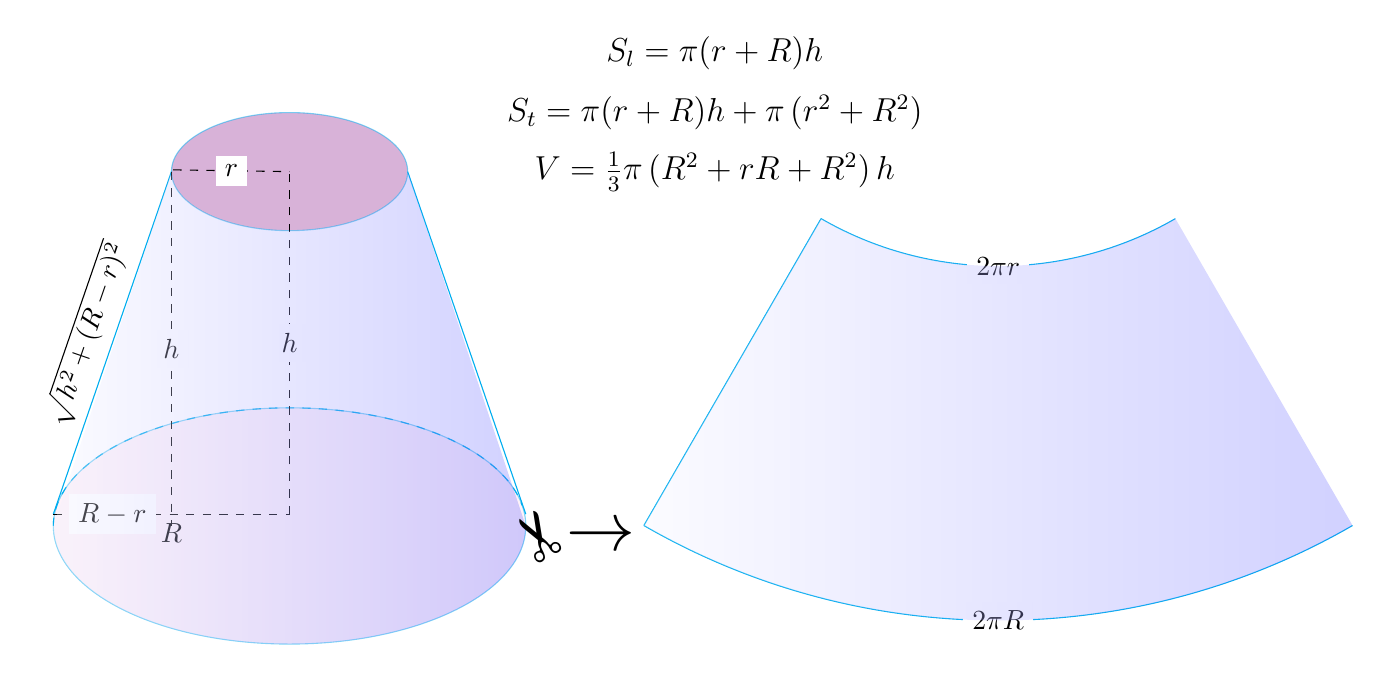
\begin{tikzpicture}[scale=1.5]
		\filldraw[cyan,fill=violet!60,opacity=.5] (0,0) ellipse(1cm and .5 cm);
		\filldraw[cyan,fill=magenta!10,opacity=.5] (0,-3) ellipse(2cm and 1 cm);
		%\draw[cyan] (-2,-3) arc (180:370:2cm and 1cm);
		\draw[cyan,dashed] (-2,-3) arc (180:10:2cm and 1cm);
		\draw[cyan] (-2,-2.9)  -- (-1,0) node[pos=.5,black,sloped,above] () {$\sqrt{h^2+(R-r)^2}$};
		\draw[cyan] (2,-2.9) -- (1,0);  
		\draw[dashed] (-1,0)--(-1,-3) node[pos=.5,fill=white] () {\bfseries $h$};
		\draw [dashed](-2,-2.9)  -- (0,-2.9) node[pos=.5,below] () {\bfseries $R$};
		\draw[dashed](0,-2.9) --(0,0) node[pos=.5,fill=white] () {\bfseries $h$};
		\draw[dashed](-0.6,0.4,) --(0,0) node[pos=.5,fill=white] () {\bfseries $r$};
		\draw (-1.5,-2.9) node[fill=white] () {\bfseries $R-r$};
		\shade[left color=blue!5!white,right color=blue!60!white,opacity=0.3] (-1,0) arc (180:360:1cm and 0.5cm) -- (2,-3) arc (360:180:2cm and 1cm) -- cycle;
		%\shade[left color=blue!5!white,right color=blue!60!white,opacity=0.3] (0,0) circle (1cm and 0.5cm);
		\draw (2.1,-3.1) node[rotate=-60] () {\Huge \Leftscissors} node[right] () {\Huge $\;\rightarrow \;$} ;
		\draw (3.6,1) node () {\large $S_l=\pi(r+R)h$};
		\draw (3.6,.5) node () {\large $S_t=\pi(r+R)h+\pi\left(r^2+R^2 \right) $};
		\draw (3.6,0) node () {\large $V=\frac{1}{3}\pi\left(R^2+rR+R^2 \right)h $};
		
		\begin{scope}[cyan,xshift=6cm,yshift=2.2cm,scale=1.5]
			\draw (-120:2cm) arc (-120:-60:2cm) node[pos=.5,black,fill=white] () {$2\pi r$};
			\draw (-120:4cm) arc (-120:-60:4cm) node[pos=.5,black,fill=white] () {$2\pi R$};
			\draw(-120:2cm) -- (-120:4cm);
			\shade[left color=blue!5!white,right color=blue!60!white,opacity=0.3] (-120:2cm) arc (-120:-60:2cm) -- (-60:4cm) arc (-60:-120:4cm) -- cycle;
		\end{scope}
	\end{tikzpicture}
\end{document}